\documentclass[xcolor=dvipsnames,table]{beamer}

\usepackage{latexsym}
\usepackage[utf8]{inputenc}
\usepackage[brazil]{babel}
\usepackage{amssymb}
\usepackage{amsmath}
\usepackage{amsfonts}
\usepackage{amsthm} 
\usepackage{newtxmath}
\usepackage{stmaryrd}
\usepackage{fancybox}
\usepackage{datetime}
\usepackage[T1]{fontenc}
\usepackage{graphicx}
\usepackage{graphics}
\usepackage{url}
\usepackage{algorithmic}
\usepackage{algorithm}
\usepackage{acronym}
\usepackage{array}
\usepackage{transparent}       
\usepackage{varioref}
\usepackage{booktabs} 
\usepackage{enumerate}
\usepackage{verbatim} 
\usepackage{multirow}
\usepackage{microtype}         
\usepackage{float}   
\usepackage{hyperref}
\usepackage{array}
\usepackage{subcaption}
\usepackage{tikz}


\newtheorem{definicao}{Definio}
\newcommand{\tab}{\hspace*{2em}}

\mode<presentation>
{
  \definecolor{colortexto}{RGB}{0,0,0}
 
  \setbeamertemplate{background canvas}[vertical shading][ bottom=white!10,top=white!10]
  \setbeamercolor{normal text}{fg=colortexto} 

  \usetheme{Madrid}
}

\title{Xunzhe Zhou's slides 1} 

\author[Xunzhe Zhou]
{\texorpdfstring{\textbf{Xunzhe Zhou} \\ Instructor: Chen, Wenbin}{Instructor: Chen, Wenbin}}

   
 \institute[]{
  Fudan University \\ School of Computer Science \\and Technology}
\date{\textbf{2020 to 2025} }

\logo{
\includegraphics[width=0.75cm]{Fudan_University_Logo.png}}

\begin{document}

	\begin{frame}
		\titlepage
	\end{frame}

	\AtBeginSection{
\begin{frame}{Summary}%[allowframebreaks]{Sumário}
    \tableofcontents[currentsection]
    %\tableofcontents[currentsection, hideothertions]
\end{frame}
	}

\begin{frame}{Summary}
	\setbeamerfont{subsection in toc}{size=\small}
	\tableofcontents
	%\tableofcontents[hideallsubsections]
\end{frame}
	
	%------------------------------------------
	
\section{Introduction}	
	\begin{frame}{Introduction}
		\begin{block}{Theorem1}{example}
   equation
		\end{block}
		%\pause
		\begin{block}{Theorem2}{example}
    equation
       \end{block}
	\end{frame}
	
	%------------------------------------------
	
\section{Main Part}
	\subsection{Part 1}{Part 1}
		\begin{frame}{Part 1}
		\begin{columns}
				\column{.6 \textwidth}  		
			\begin{block}{Theorem3}{Theorem}
			\begin{center}
				{example equation}
			\end{center}
			\end{block}		  		
		  	\begin{block}{Theorem4}{Theorem}
		  	\begin{center}
				{example equation} 
			\end{center}
			\end{block}
			\begin{block}{Theorem5}{Theorem}
			\begin{center}
				{example equation}
			\end{center}
			\end{block}
				\column{.4\textwidth}
			\begin{center}
				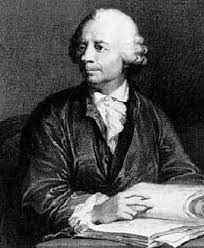
\includegraphics[height=.5\textheight]{images/euler.png}
			\end{center}	
		\end{columns}
		\end{frame}

	%------------------------------------------

\subsection{Part 2}{Part 2}
	\begin{frame}{Part 2}
		\begin{columns}
			\column{.4\textwidth} 
		\begin{center}
			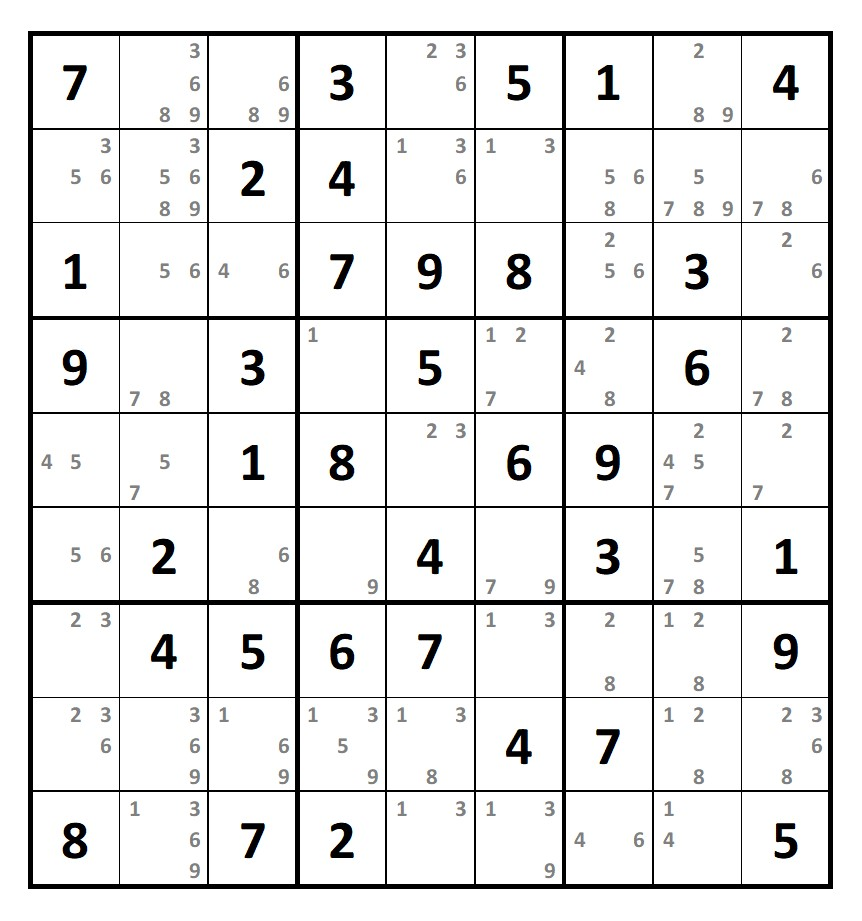
\includegraphics[height=.5\textheight]{images/imagem19.jpg}
		\end{center}
			\column{.6 \textwidth}  		
		\begin{block}{Theorem6}{Theorem}
		\begin{center}
			{example equation}
		\end{center}
		\end{block}
		\begin{block}{Theorem7}{Theorem}
		\begin{center}
			{example equation}
		\end{center}
		\end{block}
		\end{columns}
	\end{frame}	

	%------------------------------------------

\begin{frame}{Part 2}
	\begin{columns}
			\column{.4\textwidth} 
		\begin{center}
			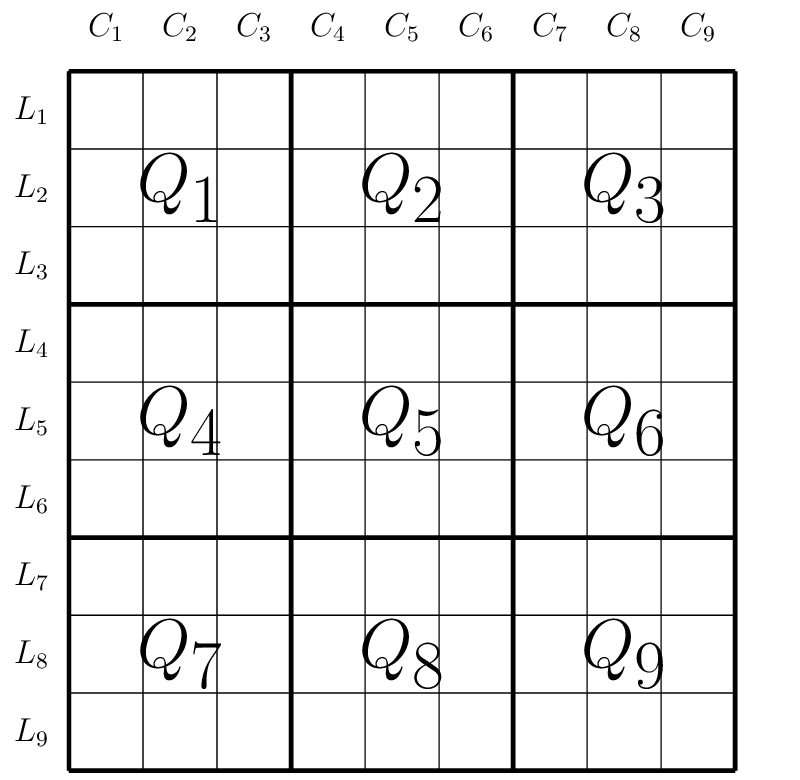
\includegraphics[height=.5\textheight]{images/imagem100.jpg}
		\end{center}
			\column{.6 \textwidth}  		
		\begin{block}{Theorem8}{Theorem}
		\begin{center}
			{example equation}
		\end{center}
		\end{block}
	\end{columns}
\end{frame}	

	%------------------------------------------

\begin{frame}{Part 2}
	\begin{columns}
			\column{.4\textwidth} 
		\begin{center}
			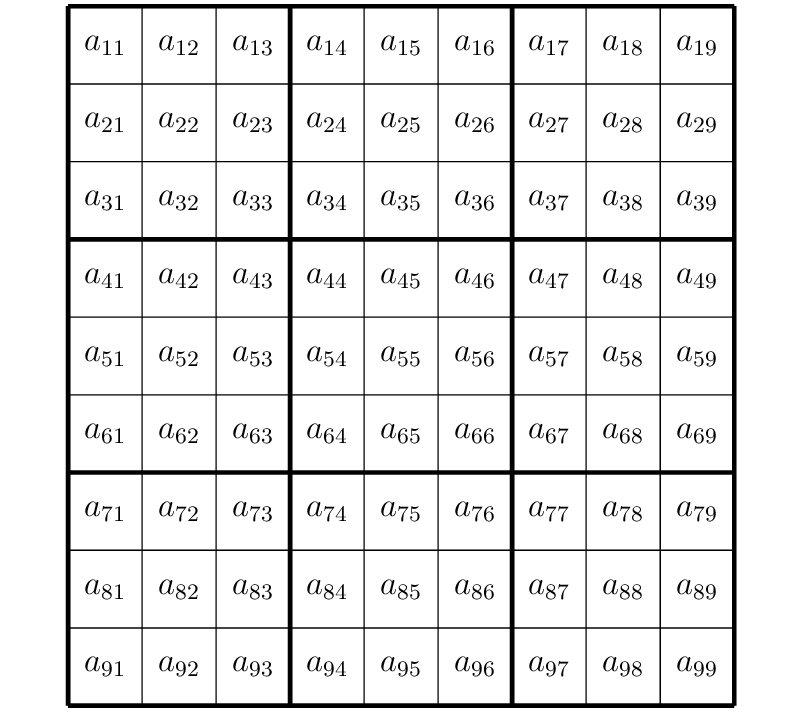
\includegraphics[height=.5\textheight]{images/imagem101.jpg}
		\end{center}
			\column{.6 \textwidth}  		
		\begin{block}{Theorem9}{Theorem}
		\begin{center}
			{example equation}
		\end{center}
		\end{block}
	\end{columns}
\end{frame}	

	%------------------------------------------
	
\subsection{Part 3}{Part 3}
	\begin{frame}{Part 3}
		\begin{columns}
			\column{.6 \textwidth}  		
		\begin{block}{Theorem10}{}
example equation
\end{block}
			\column{.4 \textwidth}  		
			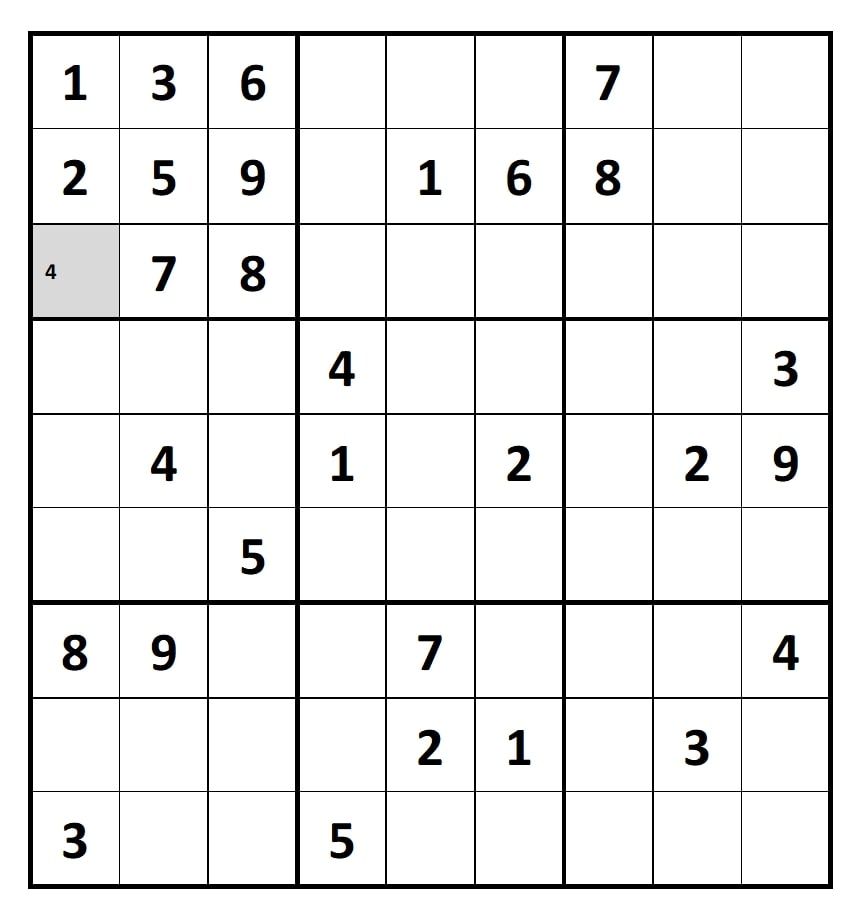
\includegraphics[width=5cm]{images/imagem20}
			%\footnotesize{Fonte: O Autor (2022).}
		\end{columns}
	\end{frame}

	%------------------------------------------

\begin{frame}{Part 3}
	\begin{columns}
		\column{.6 \textwidth}  					
	\begin{block}{Theorem11}{}
example equation
\end{block}
	\begin{block}{Theorem12}{}
example equation
\end{block}
		\column{.4 \textwidth}  		
		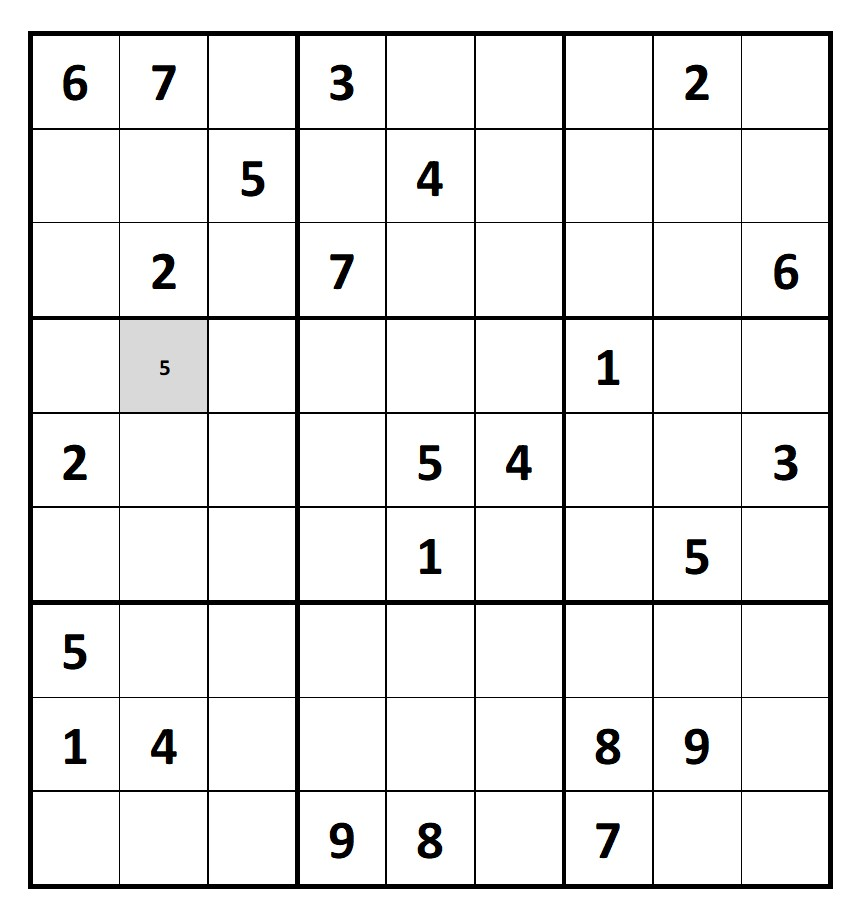
\includegraphics[width=5cm]{images/imagem21}
		%\footnotesize{Fonte: O Autor (2022).}
	\end{columns}
\end{frame}

	%------------------------------------------

\begin{frame}{Part 3}
	\begin{columns}
		\column{.6 \textwidth}  					
	\begin{block}{Theorem13}{}
example equation
\end{block}
	\begin{block}{Theorem}{}
example equation
\end{block}
		\column{.4 \textwidth}  		
		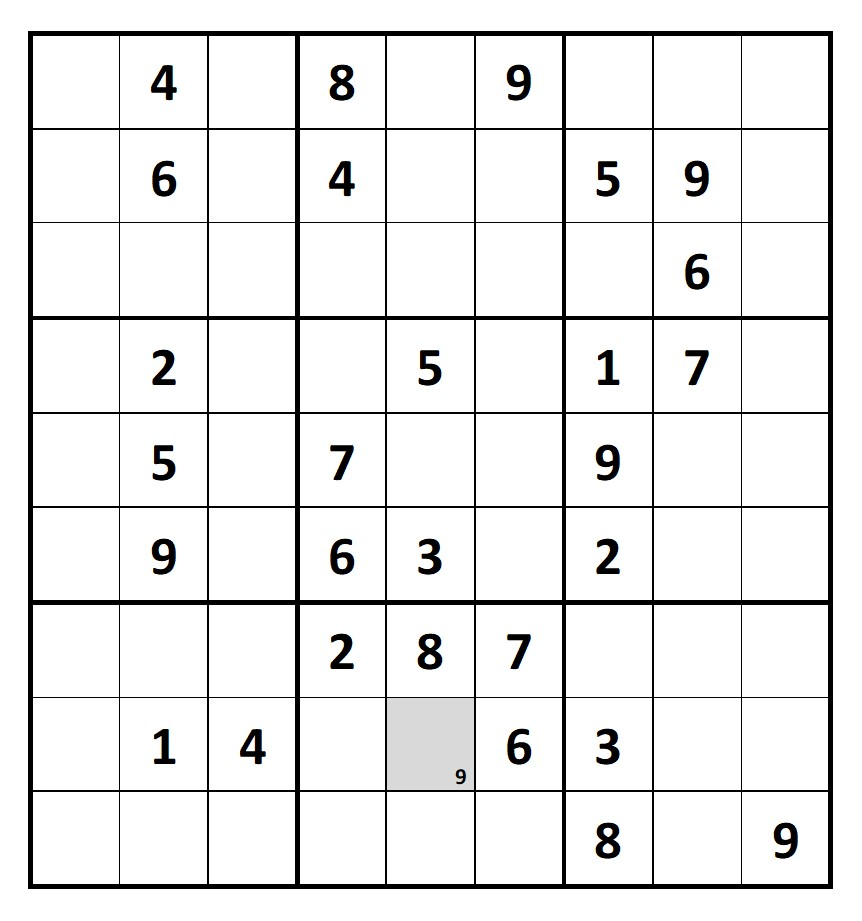
\includegraphics[width=5cm]{images/imagem22}
		%\footnotesize{Fonte: O Autor (2022).}
	\end{columns}
\end{frame}

	%------------------------------------------

\begin{frame}{Part 3}
	\begin{columns}
		\column{.6 \textwidth}  
	\begin{block}{Theorem14}{}
		example equation
	\end{block}		
	\begin{block}{Theorem15}{}
example equation
	\end{block}
		\column{.4 \textwidth}  		
		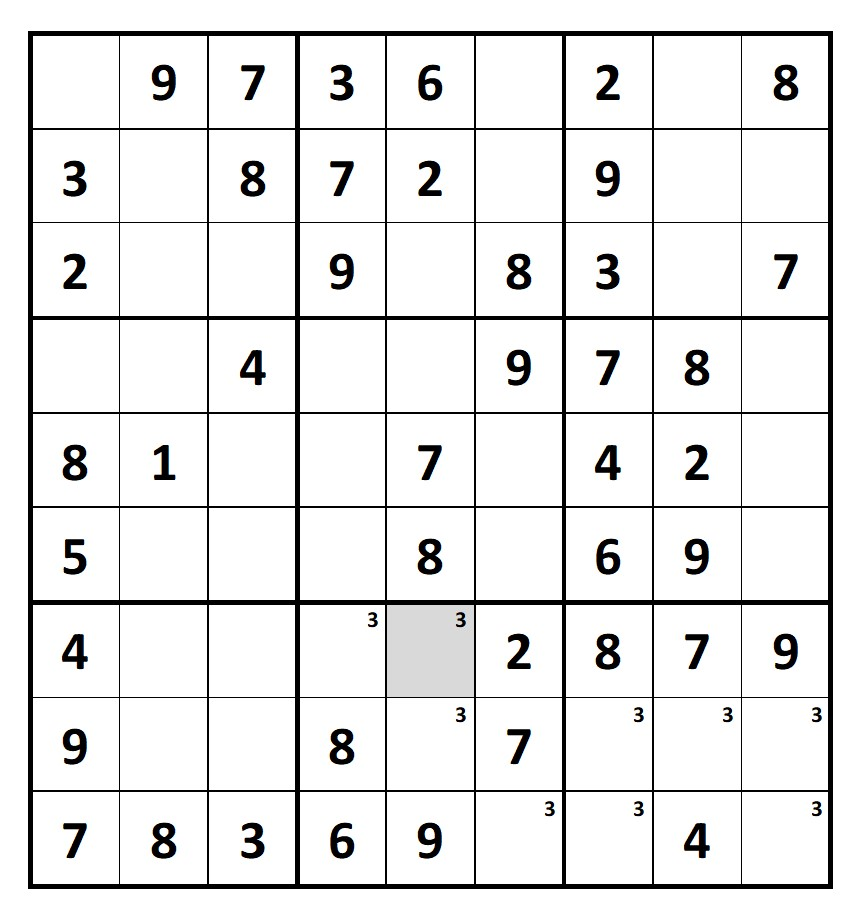
\includegraphics[width=5cm]{images/imagem23}
		%\footnotesize{Fonte: O Autor (2022).}
	\end{columns}
\end{frame}

	%------------------------------------------

\subsection{Part 4}{Part 4}
	\begin{frame}{Part 4}
		
		\begin{block}{Theorem16}{}
			example equation
		\end{block}
		\begin{alertblock}{Theorem17} 
			example equation
		\end{alertblock}
	\end{frame}

%------------------------------------------
	
\section{Reference}
	\begin{frame}{Reference}
		\begin{thebibliography}{}
			\beamertemplatearticlebibitems
			\bibitem{Lorch} Lorch, C.; Lorch, J.
			\newblock {\em Enumerating small sudoku puzzles in a first abstract algebra course}. \newblock Primus, Taylor \& Francis, v. 18, n. 2, p. 149–157, 2008.
			\beamertemplatebookbibitems
			\bibitem{West} West, D. B. et al.
			\newblock {\em Introduction to graph theory}. \newblock [S.l.]: Prentice hall Upper Saddle River,
			2001. v. 2.0.
			\beamertemplatebookbibitems
			\bibitem{Kedwewll} Keedwell, A. D.; Dénes, J.
			\newblock {\em Latin squares and their applications}. \newblock [S.l.]: Elsevier, 2015.
			\beamertemplatebookbibitems
			\bibitem{Ross} Ross, S. M.
			\newblock {\em Topics in finite and discrete mathematics}. \newblock [S.l.]: Cambridge University Press, 2000.
		\end{thebibliography}
	\end{frame}

	%------------------------------------------
	
\end{document}